\section{Multiparty Session Types}

\begin{frame}{Syntax}
  \begin{figure}[ht]
    $$\begin{array}{lclr}
        T & ::= & S & \text{(session type)} \\
          & |   & D & \text{(data type)}
      \end{array}$$

    \begin{center}
      \begin{minipage}{0.45\textwidth}
        $$\begin{array}{lclr}
            S & ::= & \texttt{end} & \text{(termination)}    \\
              & |   & L.S          & \text{(sequence)}       \\
              & |   & \mu\alpha.S  & \text{(recursion)}      \\
              & |   & \alpha       & \text{(type variable)}  \\
              & |   & (S+S)        & \text{(nondeterminism)} \\
          \end{array}$$
      \end{minipage}
      \hfill
      \begin{minipage}{0.53\textwidth}
        $$\begin{array}{lclr}
            L    & ::= & L | L                                                         & \text{(asynchrony)}   \\
                 & |   & p\rightarrow q(D)                                             & \text{(send-receive)} \\
                 & |   & \texttt{skip}                                                 & \text{(skip)}         \\
            p,q  & \in & \ZZ\cup\{\infty\}, p\ne q, pq\ge 0                            & \text{(index)}        \\
            D    & ::= & \ell | \texttt{bool} | \texttt{int} | \texttt{string} |\ldots &                       \\
            \ell & \in & \L                                                            & \text{(label)}        \\
          \end{array}$$
      \end{minipage}
    \end{center}
    % \caption{The syntax of extended multiparty session type}
    \label{syntax}
  \end{figure}
\end{frame}

\begin{frame}{Operational Semantics}
  $$\begin{array}{lr}
      L.S \xrightarrow{\makebox[1cm][c]{L}} S
                                                      & \text{(sequence)}       \\
      \mu\alpha.S
      \xrightarrow{\makebox[1cm][c]{\texttt{skip}}} \alpha
      \xrightarrow{\makebox[1cm][c]{\texttt{skip}}} S & \text{(recursion)}      \\

      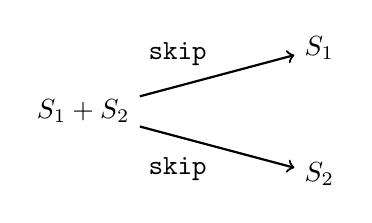
\begin{tikzpicture}[baseline={(current bounding box.center)}, ->, thick]
        \node (src) at (0,0) {\( S_1 + S_2 \)};
        \node (tgt1) at (3,0.8) {\( S_1 \)};
        \node (tgt2) at (3,-0.8) {\( S_2 \)};

        \draw[->] (src) -- node[above left] {\texttt{skip}} (tgt1);
        \draw[->] (src) -- node[below left] {\texttt{skip}} (tgt2);
      \end{tikzpicture}

                                                      & \text{(nondeterminism)} \\
    \end{array}$$
  \textbf{Note:}
  \begin{itemize}
    \item A type $S$ generates a directed graph (NFA) $\text{gr}(S)$ called a semantic graph, with an initial node and the terminal node $\texttt{end}$. We can rename the nodes for convenience.
    \item From the graph, we can show commutativity and distributivity of nondeterminism. Hence we can just write $S_1+S_2+S_3$ instead of $(S_1+S_2)+S_3$.
    \item Conversely, for each directed graph whose edges are defined by the production rules for $L$ (can have multiple terminal nodes), we have a type.
  \end{itemize}



\end{frame}

\begin{frame}{Subtype}
  We want to encode in our type system
  \begin{itemize}
    \item Determinism is allowed in a nondeterministic context
          $$S_1\preceq S_1+S_2.$$
    \item Waiting for more actions to be asynchronously executed is allowed
          $$L_1|L_2 \preceq L_1.$$
  \end{itemize}

  The latter can be expressed as a relation between two \textit{edges}.
\end{frame}

\begin{frame}{Trace and Path}
  A path is a sequence $S_1\xrightarrow{L_1}S_2\xrightarrow{L_2}\cdots\xrightarrow{L_n}\texttt{end}$. Given this path, we have a trace $t=L_1.L_2 \ldots L_n$. The length of $t$ is $|t|=n$.

  A trace $t=L_1.L_2 \ldots L_n$ is equivalent to the path from $t$ removing a \texttt{skip}
  $$L_1.L_2 \ldots L_n \equiv L_1\ldots L_{j-1}.L_j\ldots L_n \text{ if } L_j = \texttt{skip}.$$

  Let $t=L_1.L_2 \ldots L_n$ and $t'=L'_1.L'_2 \ldots L'_n$. Define $t\preceq t'$ if $L_i\preceq L'_i$ for all $i\in\{1,\ldots,n\}$.

  Let $t_1$ and $t_2$ be two traces. Then $t_1\preceq t_2$ if there exist $t'_1$ and $t'_2$ of the same length such that $t_1 \equiv t'_1$, $t_2 \equiv t'_2$ and $t'_1\preceq t'_2$.
\end{frame}

\begin{frame}{Subtype}
  Hence we can define subtype relation based on generated graphs.

  Let $\text{tr}(S)$ the set of traces of the graph generated by $S$.

  We define $S_1\preceq S_2$ if for any $t_1\in\text{tr}(S_1)$, there exists $t_2\in\text{tr}(S_2)$ such that $t_1\preceq t_2$.

  But the best thing we should do is to derive equational reasoning on types.

  \begin{itemize}
    \item For each type $S$, there exists a corresponding \textit{regular expression}.
    \item There have been proof theories on regular expressions (Kleen algebra) and right-linear grammar \footnote{Das, Anupam, and Abhishek De. "A proof theory of right-linear ($\omega$-) grammars via cyclic proofs." Proceedings of the 39th Annual ACM/IEEE Symposium on Logic in Computer Science. 2024.}
  \end{itemize}
\end{frame}

\begin{frame}{Projection}
  \begin{center}
    \begin{minipage}{0.48\textwidth}
      $$\begin{array}{rlr}
          p\rightarrow q \downharpoonright_p & =

          \begin{cases}
            0\rightarrow \infty, & \text{ if } q=0   \\
            0\rightarrow -q,     & \text{ if } q < 0 \\
            \varnothing,         & \text{ otherwise} \\
          \end{cases}
        \end{array}$$
    \end{minipage}
    \hfill
    \begin{minipage}{0.48\textwidth}
      $$\begin{array}{rlr}
          q\rightarrow p \downharpoonright_p & =
          \begin{cases}
            \infty\rightarrow 0, & \text{ if } q=0   \\
            -q\rightarrow 0,     & \text{ if } q < 0 \\
            \varnothing,         & \text{ otherwise} \\
          \end{cases}
        \end{array}$$
    \end{minipage}
  \end{center}

  $$\begin{array}{rlr}
      L_1|L_2 \downharpoonright_p           & =
      L_1\downharpoonright_p | L_2 \downharpoonright_p                                                   \\
      \texttt{skip}\downharpoonright_p      & = \texttt{skip}                                            \\

      p\rightarrow q (D)\downharpoonright_p & =
      \begin{cases}
        p\rightarrow q\downharpoonright_p (D), \text{ if } p\rightarrow q\downharpoonright_p\ne\varnothing \\
        \texttt{skip}, \text{ otherwise}
      \end{cases} \\
    \end{array}$$

  From $\text{gr}(S)$, we replace each edge by its projection. The type derived from this graph is the projected type $S\downharpoonright_p$.

  \textbf{Proposition:} If $S_1\preceq S_2$, then $S_1\downharpoonright_p \preceq S_2\downharpoonright_p,\forall p \in \NN^{-}$.
\end{frame}

